\chapter{Results and Discussion} % Main chapter title

\label{Chapter5} % Change X to a consecutive number; for referencing this chapter elsewhere, use \ref{ChapterX}

\section{Solvation free energies}

The first part of this work consisted of obtaining phenanthrene parameters for the SAFT-$\gamma$ Mie Force Field as described in section \ref{parame}. This part was necessary since these parameters were not available for the ring geometry on the force field database. The parameters obtained and the mean percentage error (MPE) to the experimental data \cite{pvphen} were:

\begin{table*}[h]
    \centering
    \caption{Estimated SAFT-$\gamma$ Mie Force Field parameters for phenanthrene.}
    \label{tbl:estimparameters}
    \begin{tabular}{lllll}
    	\hline\hline
    	$m_s$                & $\epsilon/k_{B}$ (K) & $\sigma (\dot{A})$ & $\lambda_r$ & MPE(\%)   \\ \hline
    	3 \cite{lafitte2012} & 485.55               & 4.197              & 14.34       & 1.64|9.74 \\
    	5  \cite{muller2017} & 262.74               & 4.077              & 9.55        & 0.88      \\ \hline\hline
    \end{tabular}
    
\end{table*} 

In the table above, the first value of MPE for the \citeonline{lafitte2012} strategy corresponds to the estimation with experimental data and the second corresponds to the corrections factors estimation with MD data. This strategy has an inconsistency since parameters solely estimated with the EoS do not perform well in molecular simulations. Hence, we only studied the solvation free energy of phenanthrene with the set of parameters estimated with \citeonline{muller2017} strategy. In fact, we only followed the \cite{lafitte2012} strategy because it was the sole one available when we first started this work. The sets of parameters for the other compounds were retrieved from the literature \cite{lobanova2016,herdes2015,ervik2016,muller2017}, and all the utilized parameters are available in Table \ref{tbl:parameters}.

\begin{table*}[h]
\centering
  \caption{SAFT-$\gamma$ Mie Force Field for each substance used in this work.}
  \label{tbl:parameters}
  \begin{tabular}{lllll}
      \hline
      \hline
                     & $m_s$ & $\epsilon/k_{B}$ (K) & $\sigma (\dot{A})$ & $\lambda_r$ \\ \hline
      Water          & 1     & 305.21               & 2.902              & 8.0         \\
      Propane        & 1     & 426.08               & 4.871              & 34.29       \\
      Carbon dioxide & 2     & 194.94               & 2.848              & 14.65       \\
      Hexane         & 2     & 376.35               & 4.508              & 19.57       \\
      Octanol        & 3     & 495.71               & 4.341              & 28.79       \\
      Toluene        & 3     & 268.24               & 3.685              & 11.80       \\
      Benzene        & 3     & 230.30               & 3.441              & 10.45       \\
      Pyrene         & 4     & 459.04               & 4.134              & 15.79       \\
      Anthracene     & 5     & 259.68               & 3.631              & 9.55        \\ 
      \hline
      \hline
  \end{tabular}

\end{table*}
\FloatBarrier
The solvation free energies of aromatic solutes in nonpolar (hexane), aromatic (toluene) and hydrogen bonding (1-octanol) solvents were examined with binary interaction parameters equal to zero. Since the force field does not account for charges, we only needed to calculate the Mie contribution ( Eq. \eqref{eq:softcore}) to the solvation free energy. A total of 15-18 $\lambda s$, depending on the pairs solute-solvent,   and their respective $\eta s$ were estimated as described in the methodology. The final $\lambda$ set was found using  the cumulative probability distribution (Eq. \eqref{eqn:cumfun}) for all pairs. The distribution for the pair hexane+benzene can be seem in \figref{fig:optimized_cdf} and the optimized values of $\lambda$ and $\eta$ in Table \ref{tbl:lambdahex}. The $\lambda s$ and $\eta s$  for the other pairs are available at  Appendix A. Observing the coupling parameters found for all the pairs, we can see that they are concentrated on the region with a steeper slope as it is expected by this method.

\begin{figure}[h]
\centering
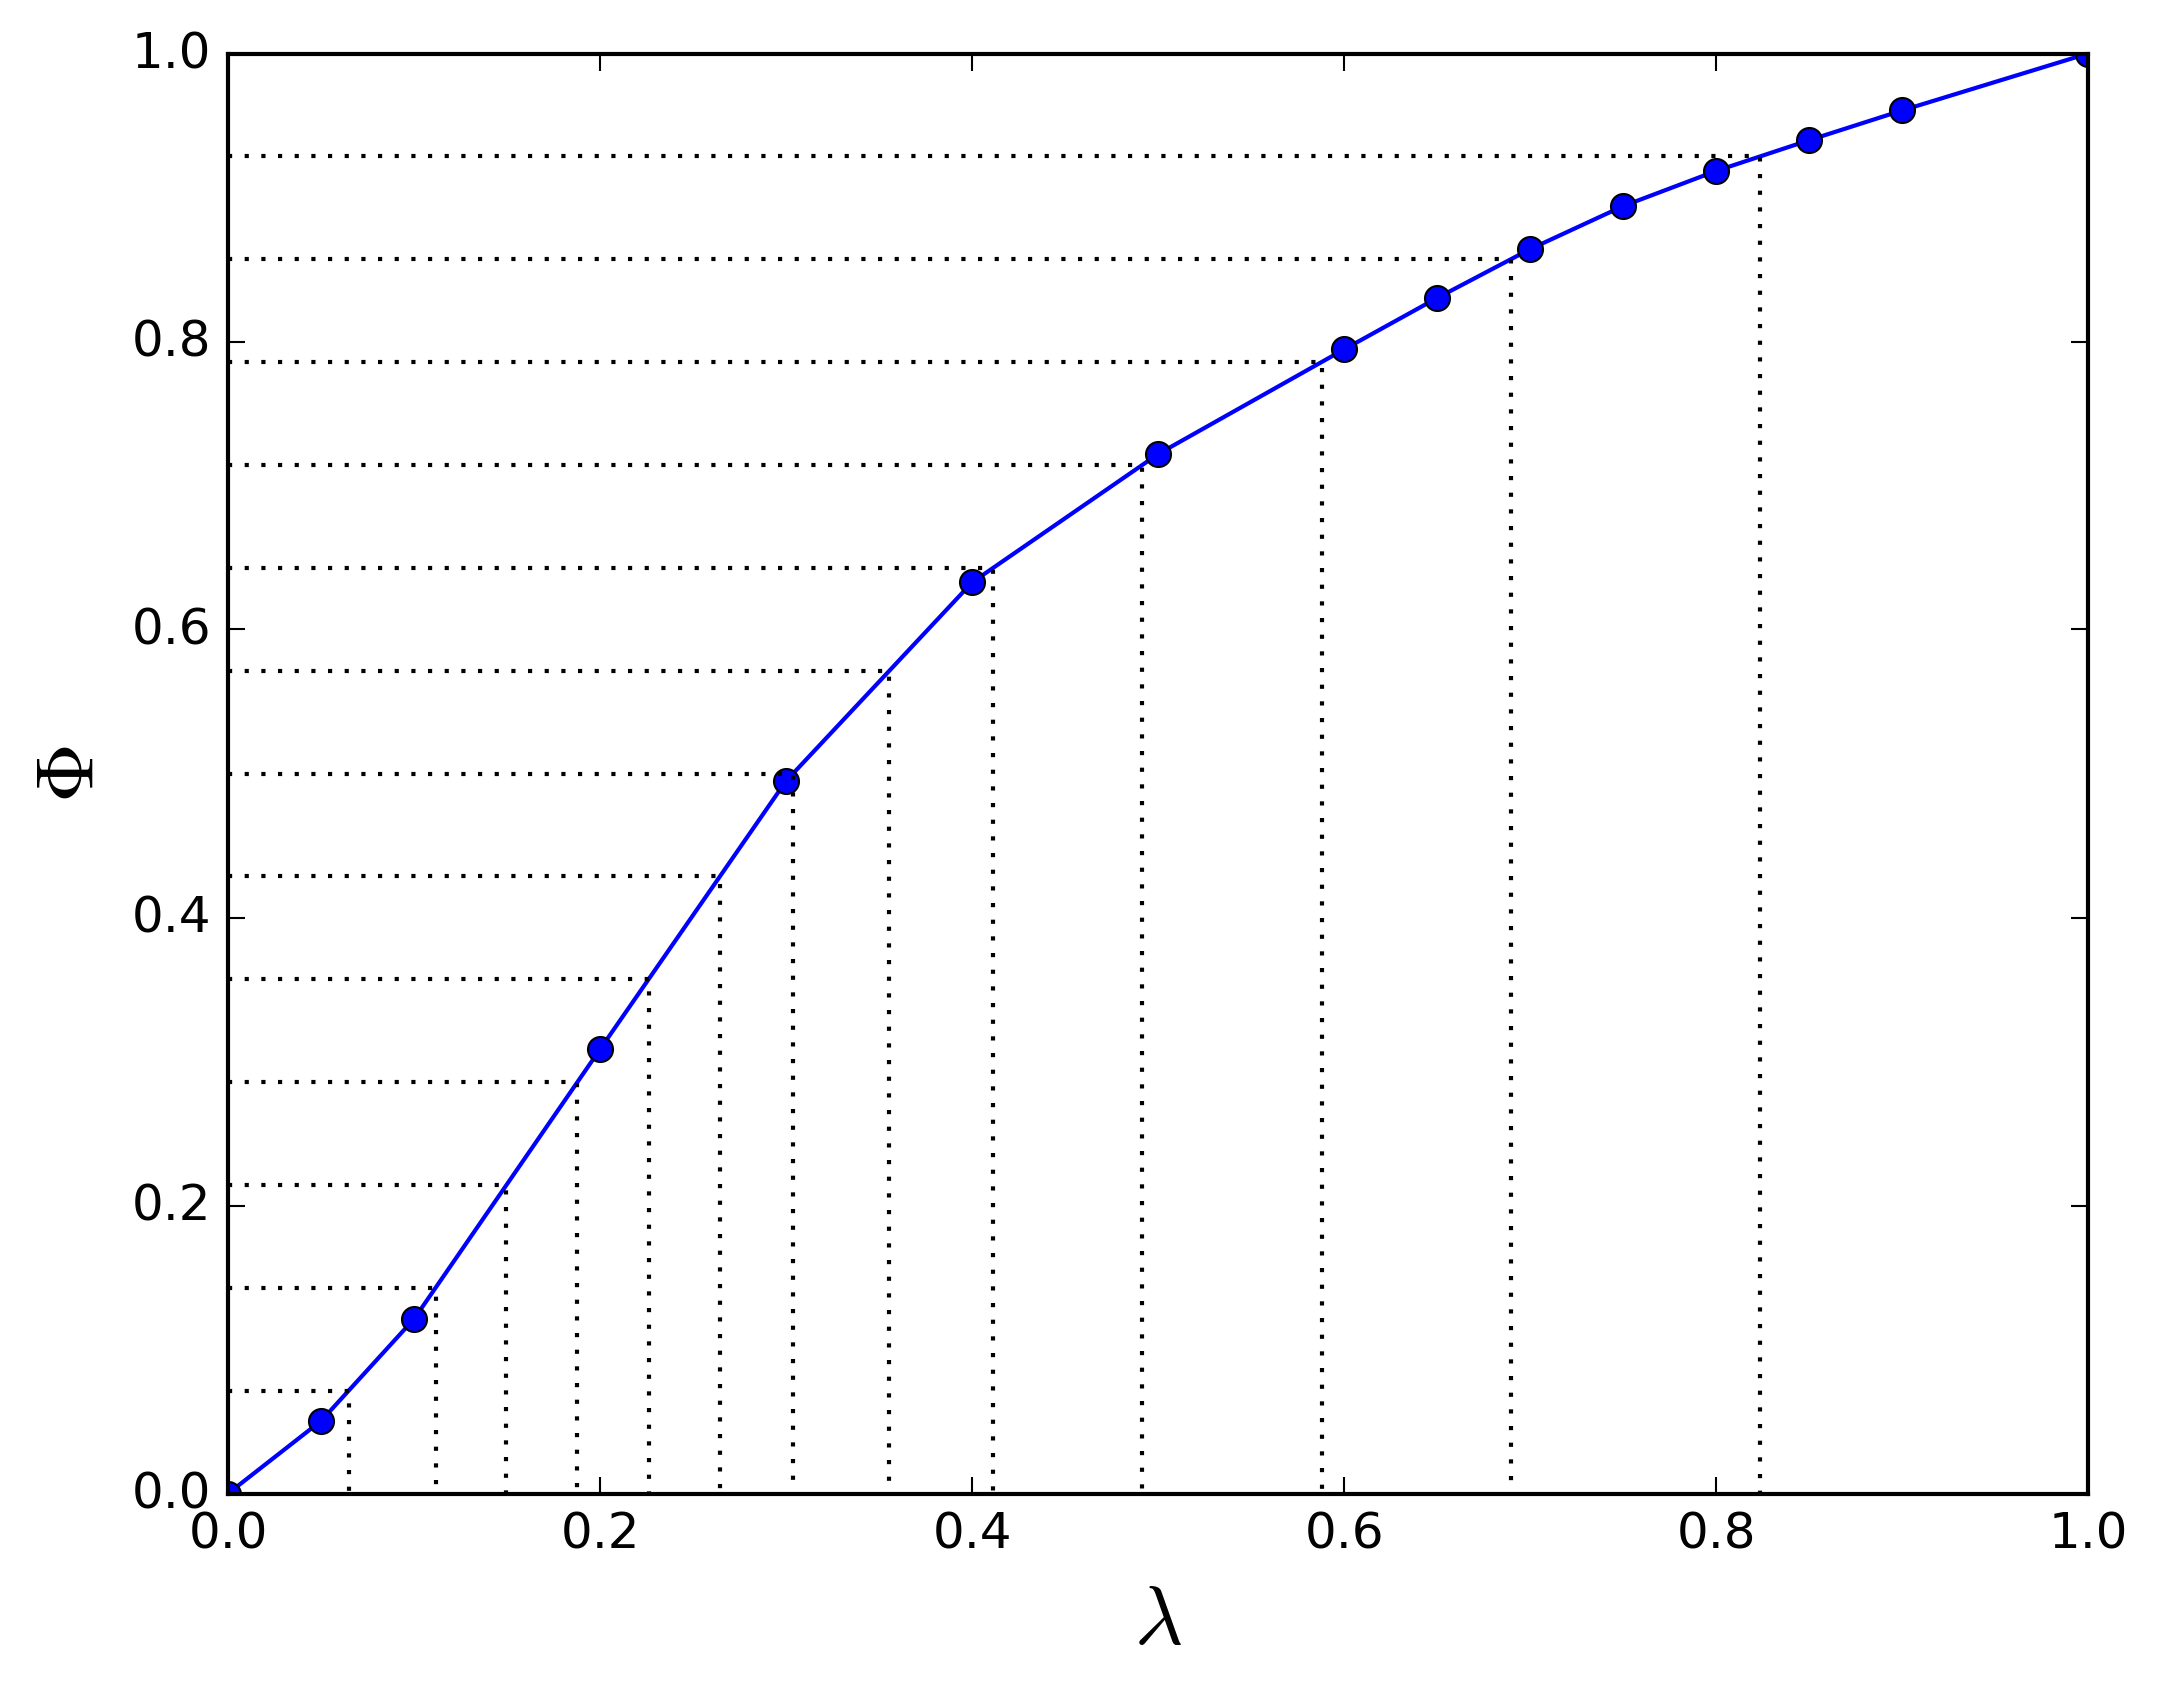
\includegraphics[width=0.7\linewidth]{Figures/optimized_cdf}
\caption{Cumulative probability}
\label{fig:optimized_cdf}
\end{figure}

\begin{table*}[h]
    \centering
    \caption{Optimized values of $\lambda$ and $\eta$ for the pair benzene + hexane.}
      \label{tbl:lambdahex}
    \begin{tabular}{ll}
    	\hline\hline
    	$\lambda$ & $\eta$ \\ \hline
    	0         & 0      \\
    	0.065     & 0.708  \\
    	0.112     & 1.385  \\
    	0.15      & 1.892  \\
    	0.188     & 2.399  \\
    	0.226     & 2.519  \\
    	0.264     & 2.457  \\
    	0.304     & 2.367  \\
    	0.356     & 1.921  \\
    	0.411     & 1.411  \\
    	0.492     & 0.524  \\
    	0.588     & -0.663 \\
    	0.69      & -2.016 \\
    	0.824     & -3.922 \\
    	1         & -6.583 \\ \hline\hline
    \end{tabular}
\end{table*}
\FloatBarrier
It is also important to analyze the reliability of solvation free energy estimations  through the overlapping of the intermediate states. Insufficient overlap among states when using FEP based methods such as MBAR may result in the underestimation of variance, and, consequently, in substantially incorrect free energies \cite{klimovich}. The overlapping matrix for the solvation free energy of benzene in hexane is presented in \figref{fig:hexove} and the matrices for the other pairs are available at Appendix B. The elements of these matrices are the probabilities of observing a sample from state  i in state j. As an example, the probability of observing state 6 in a simulation of state 8 is 0.16 in \figref{fig:hexove}. It can be observed in the figures that  the matrices for all the pairs in this work have more than  three diagonals. In addition to that,  the probabilities in the three main diagonals are higher than 0.03, which are one of the characteristics of a reliable free energy estimation \cite{klimovich}. After this analysis, we present in Table \ref{tbl:solv1} the results for solvation free energy calculations and the absolute deviations to experimental data \cite{doi:10.1021/ci034120c}.   

\FloatBarrier
\begin{figure}[h]
    \centering
    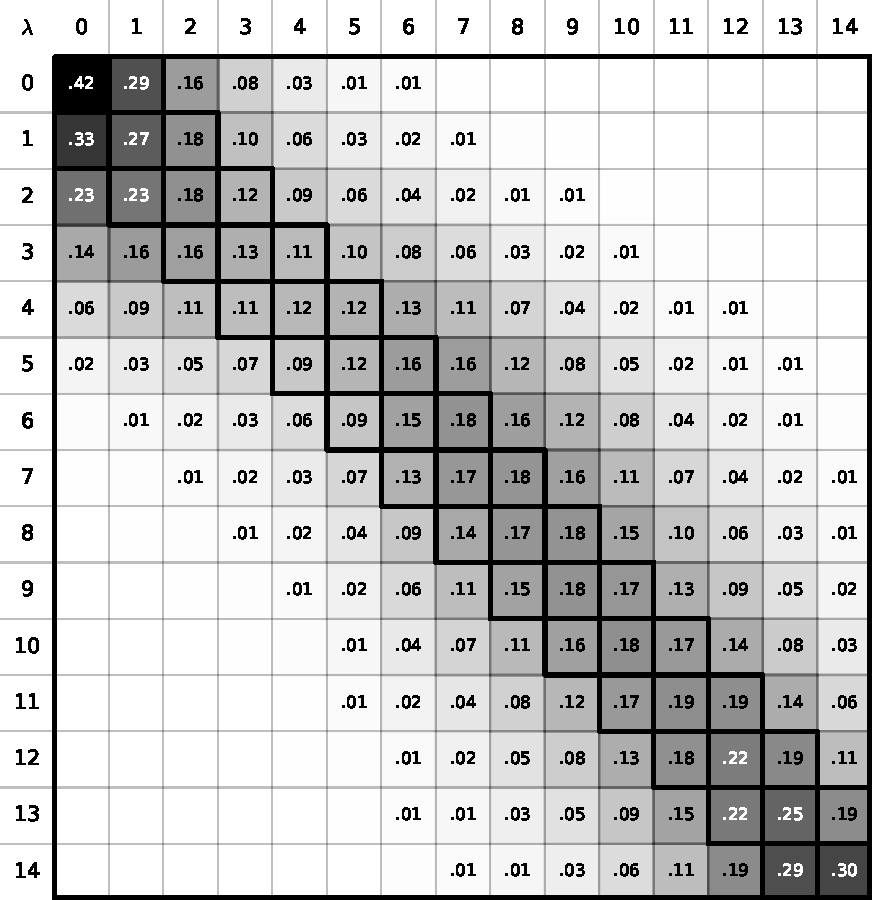
\includegraphics[width=0.8\textwidth]{Figures/ohex_benz}
    \caption{Overlapping matrix for hexane+benzene.}
    \label{fig:hexove}
\end{figure}

\begin{table*}[h]
\centering
  \caption{Calculated and experimental values for the solvation free energy differences (kcal/mol) of solutes in non aqueous solvents.}
  \label{tbl:solv1}
  \begin{tabular}{lllll}
  	\hline\hline
  	Solvent               & Solute       & $\Delta G_{solv}^{exp}$ & $\Delta G_{solv}^{Mie}$ & Absolute  \\
  	                      &              &                         &                         & Deviation \\ \hline
  	hexane                & benzene      & -3.96                   & -3.76  $\pm$ 0.01       & 0.20      \\
  	hexane                & pyrene       & -11.53                  & -10.82 $\pm$ 0.02       & 0.71      \\
  	hexane                & phenanthrene & -10.01                  & -9.16  $\pm$ 0.01       & 0.85      \\
  	1-octanol             & propane      & -1.32                   & -1.36  $\pm$ 0.02       & 0.04      \\
  	1-octanol             & anthracene   & -11.72                  & -8.16  $\pm$ 0.03       & 3.61      \\
  	1-octanol             & phenanthrene & -10.22                  & -8.34  $\pm$ 0.03       & 1.47      \\
  	toluene               & pyrene       & -12.86                  & -11.74 $\pm$ 0.01       & 1.11      \\
  	toluene               & anthracene   & -11.31                  & -9.90 $\pm$ 0.01        & 1.41      \\
  	%    \hline
%    RMSE &              &                         &                         & 1.48      \\ \hline\hline
  \end{tabular}
\end{table*}
\FloatBarrier

The numerical values for solvation free energies in hexane had smaller absolute deviations to experimental data, what shows that the SAFT-$\gamma$ Mie force field performs better for a non-polar solvent. Additionally, this force field presented better results for the pair hexane+benzene than the Trappe force field (- 4.35  $\pm$ 0.05 kcal/mol) \cite{garrido2011} and the ELBA coarse-grained force field  (-2.92 $\pm$ 0.01 kcal/mol) \cite{doi:10.1021/acs.jctc.5b00963}. We also observed the effect of molecule's size on the entropic region of the free energy curve in Figure \ref{fig:hex}. It was expected that a force field based on an EoS that does not explicitly account for hydrogen bond would not perform well for 1-octanol. Despite this, the solvation free energies of propane and phenanthrene in 1-octanol stayed in the desired deviation range of 1-2 kcal/mol \cite{doimobley}. The solvation free energy absolute deviation for propane was much smaller when compared to the other solutes, what can be attributed to propane's non-polarity and smoother free energy curve (Figure \ref{fig:oct}). This solvation free energy of propane in 1-octanol also had a smaller deviation than the prediction of the ELBA force field (-0.92 $\pm$ 0.01) \cite{doi:10.1021/acs.jctc.5b00963}. The anthracene and phenanthrene molecules have the same geometry in the model and similar physical properties, but the absolute deviation of the solvation free energy of anthracene in 1-octanol is much higher than the one of phenanthrene 1-octanol. This high deviation may indicate a problem in the parameterization of anthracene.      

\begin{figure}[H]
\centering
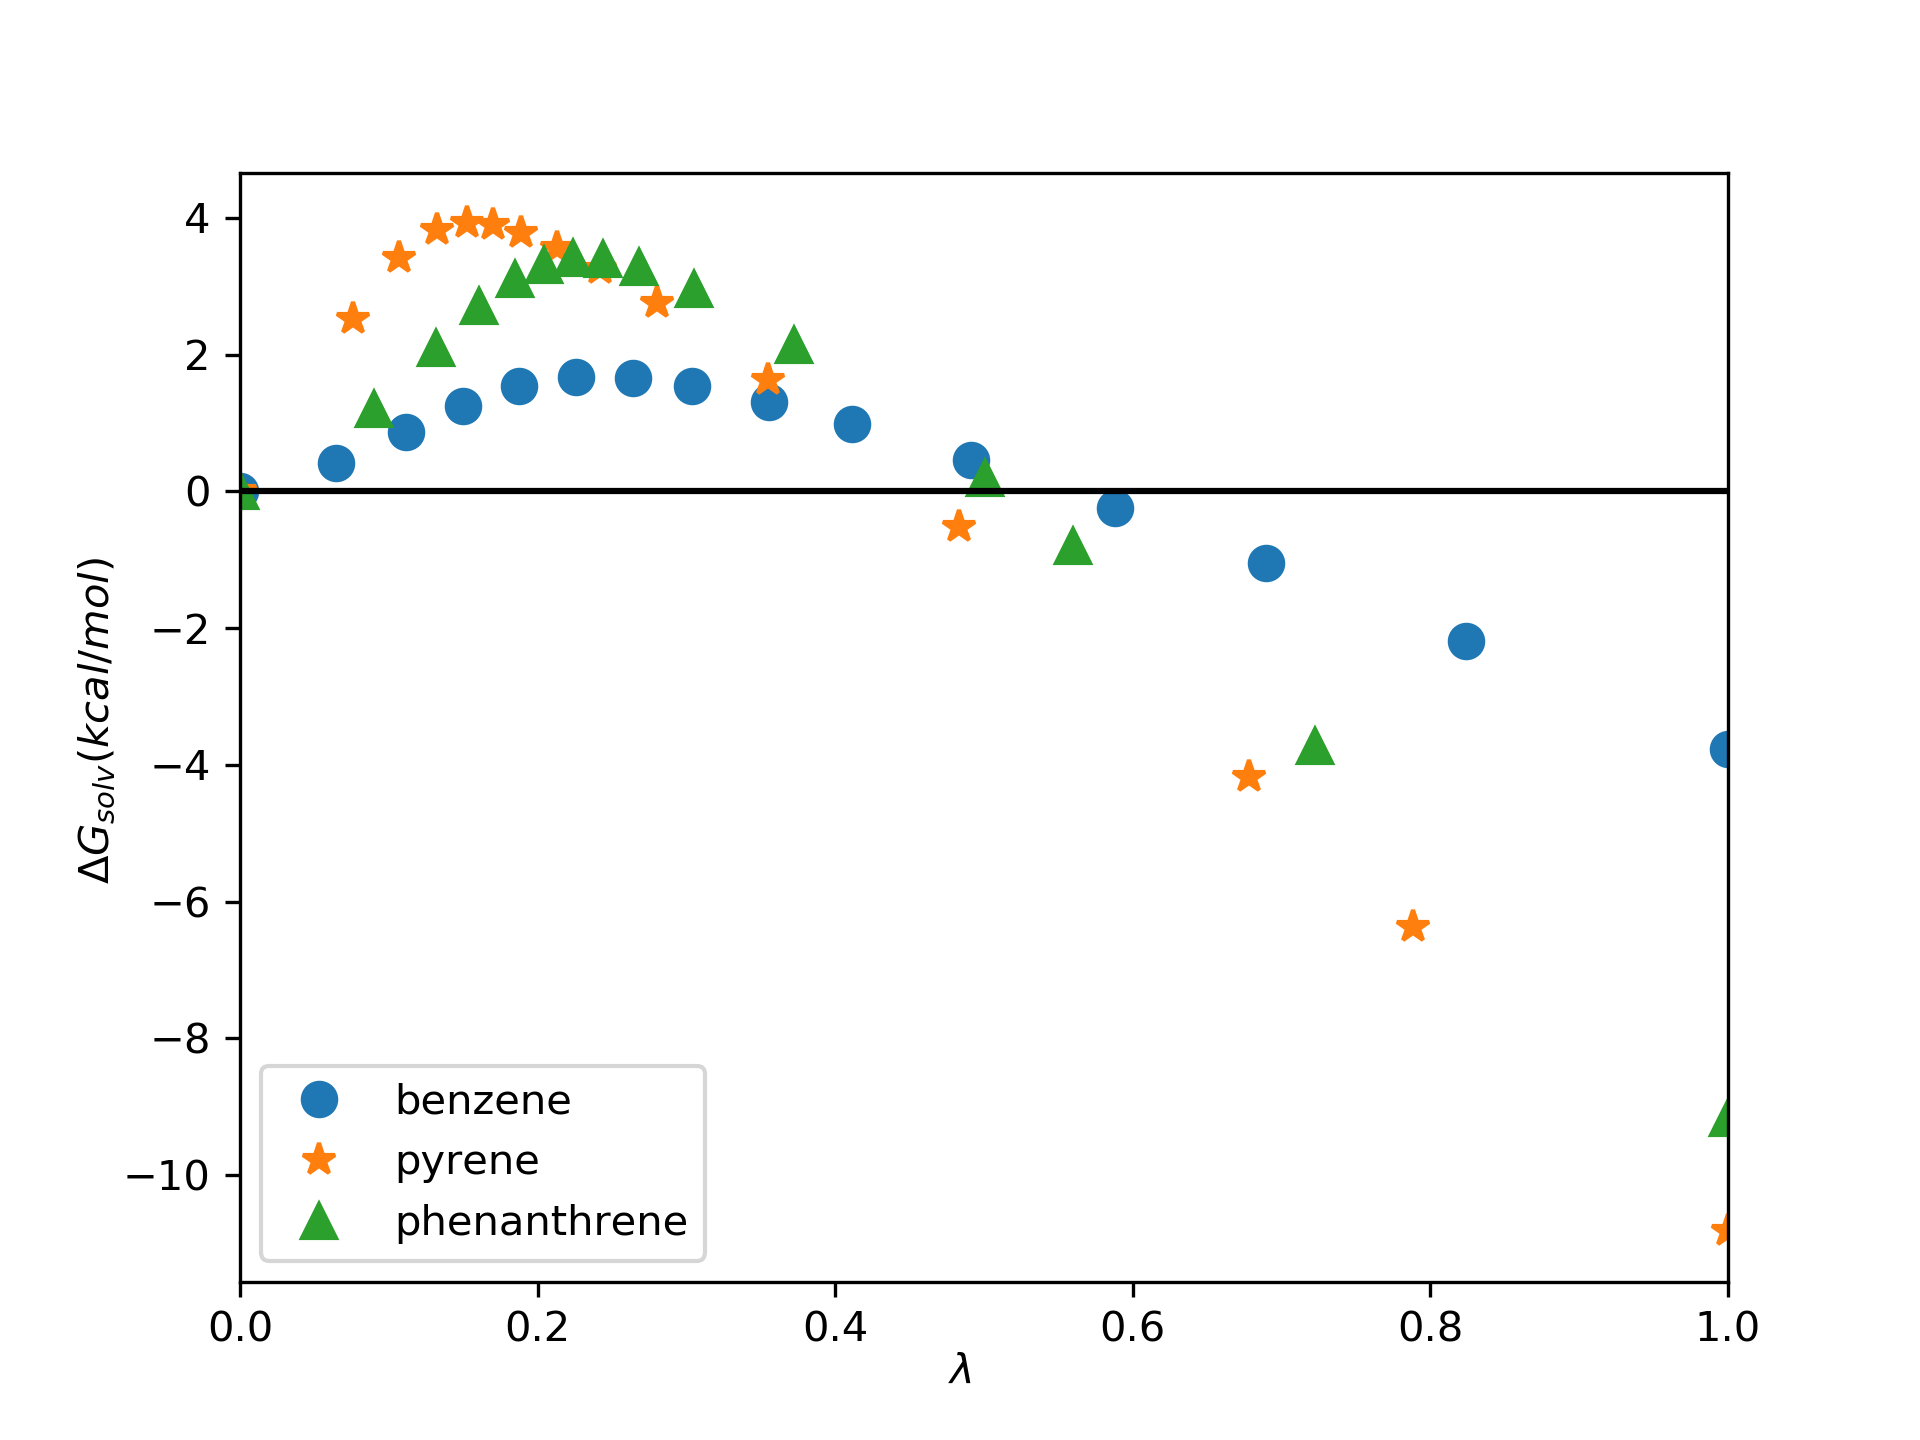
\includegraphics[width=0.9\linewidth]{Figures/hex}
\caption{Solvation free energy profiles of different solutes in hexane.}
\label{fig:hex}
\end{figure}

\begin{figure}[H]
    \centering
    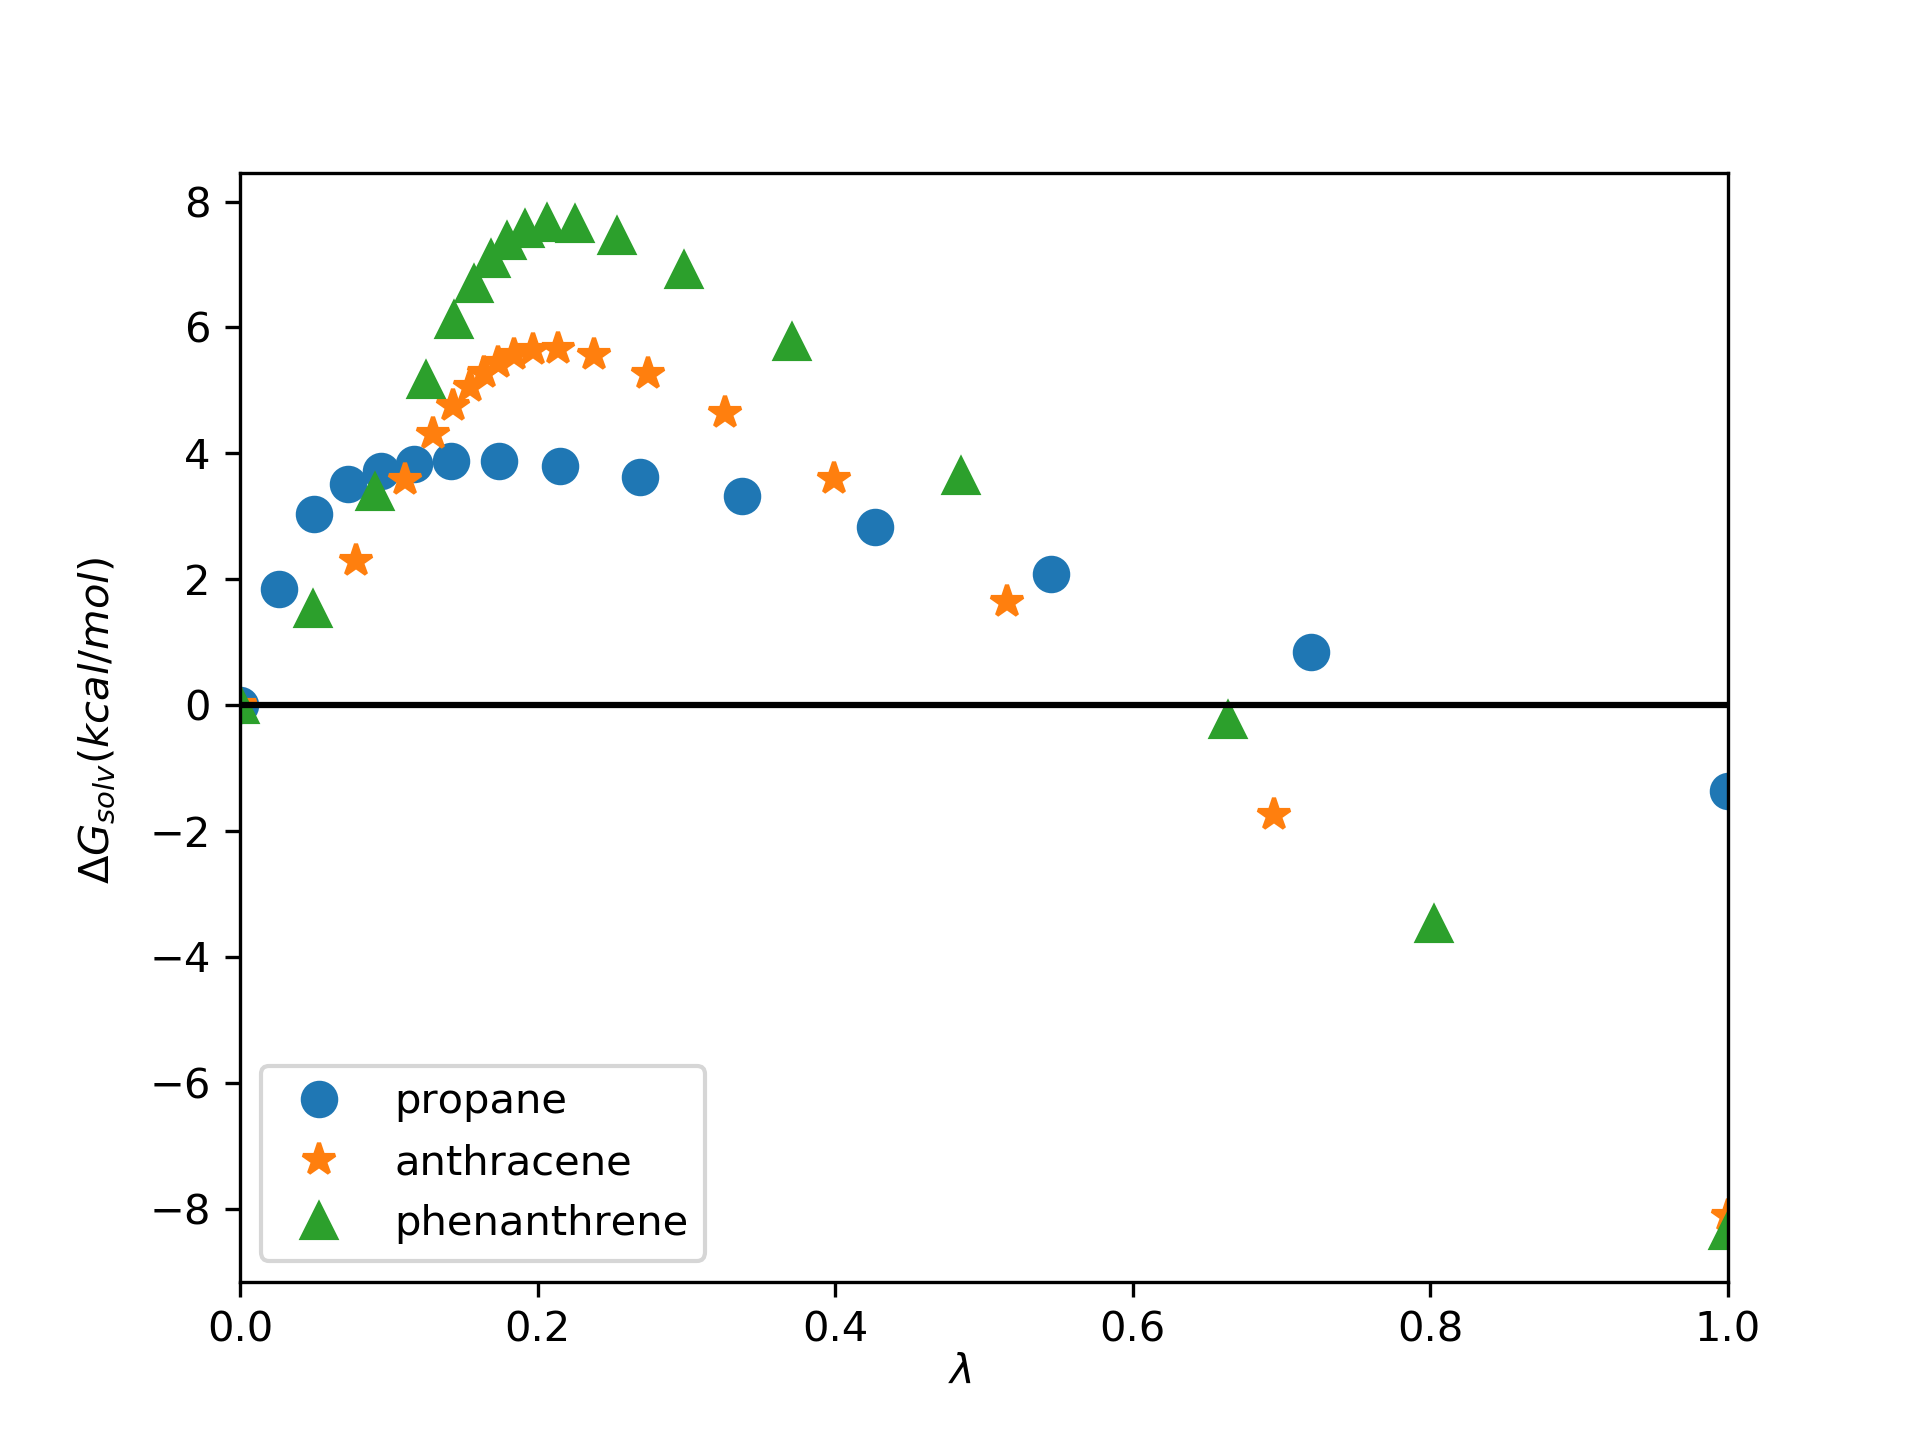
\includegraphics[width=0.9\linewidth]{Figures/oct}
    \caption{Solvation free energy profiles of different solutes in 1-octanol.}
    \label{fig:oct}
\end{figure}

\begin{figure}[H]
    \centering
    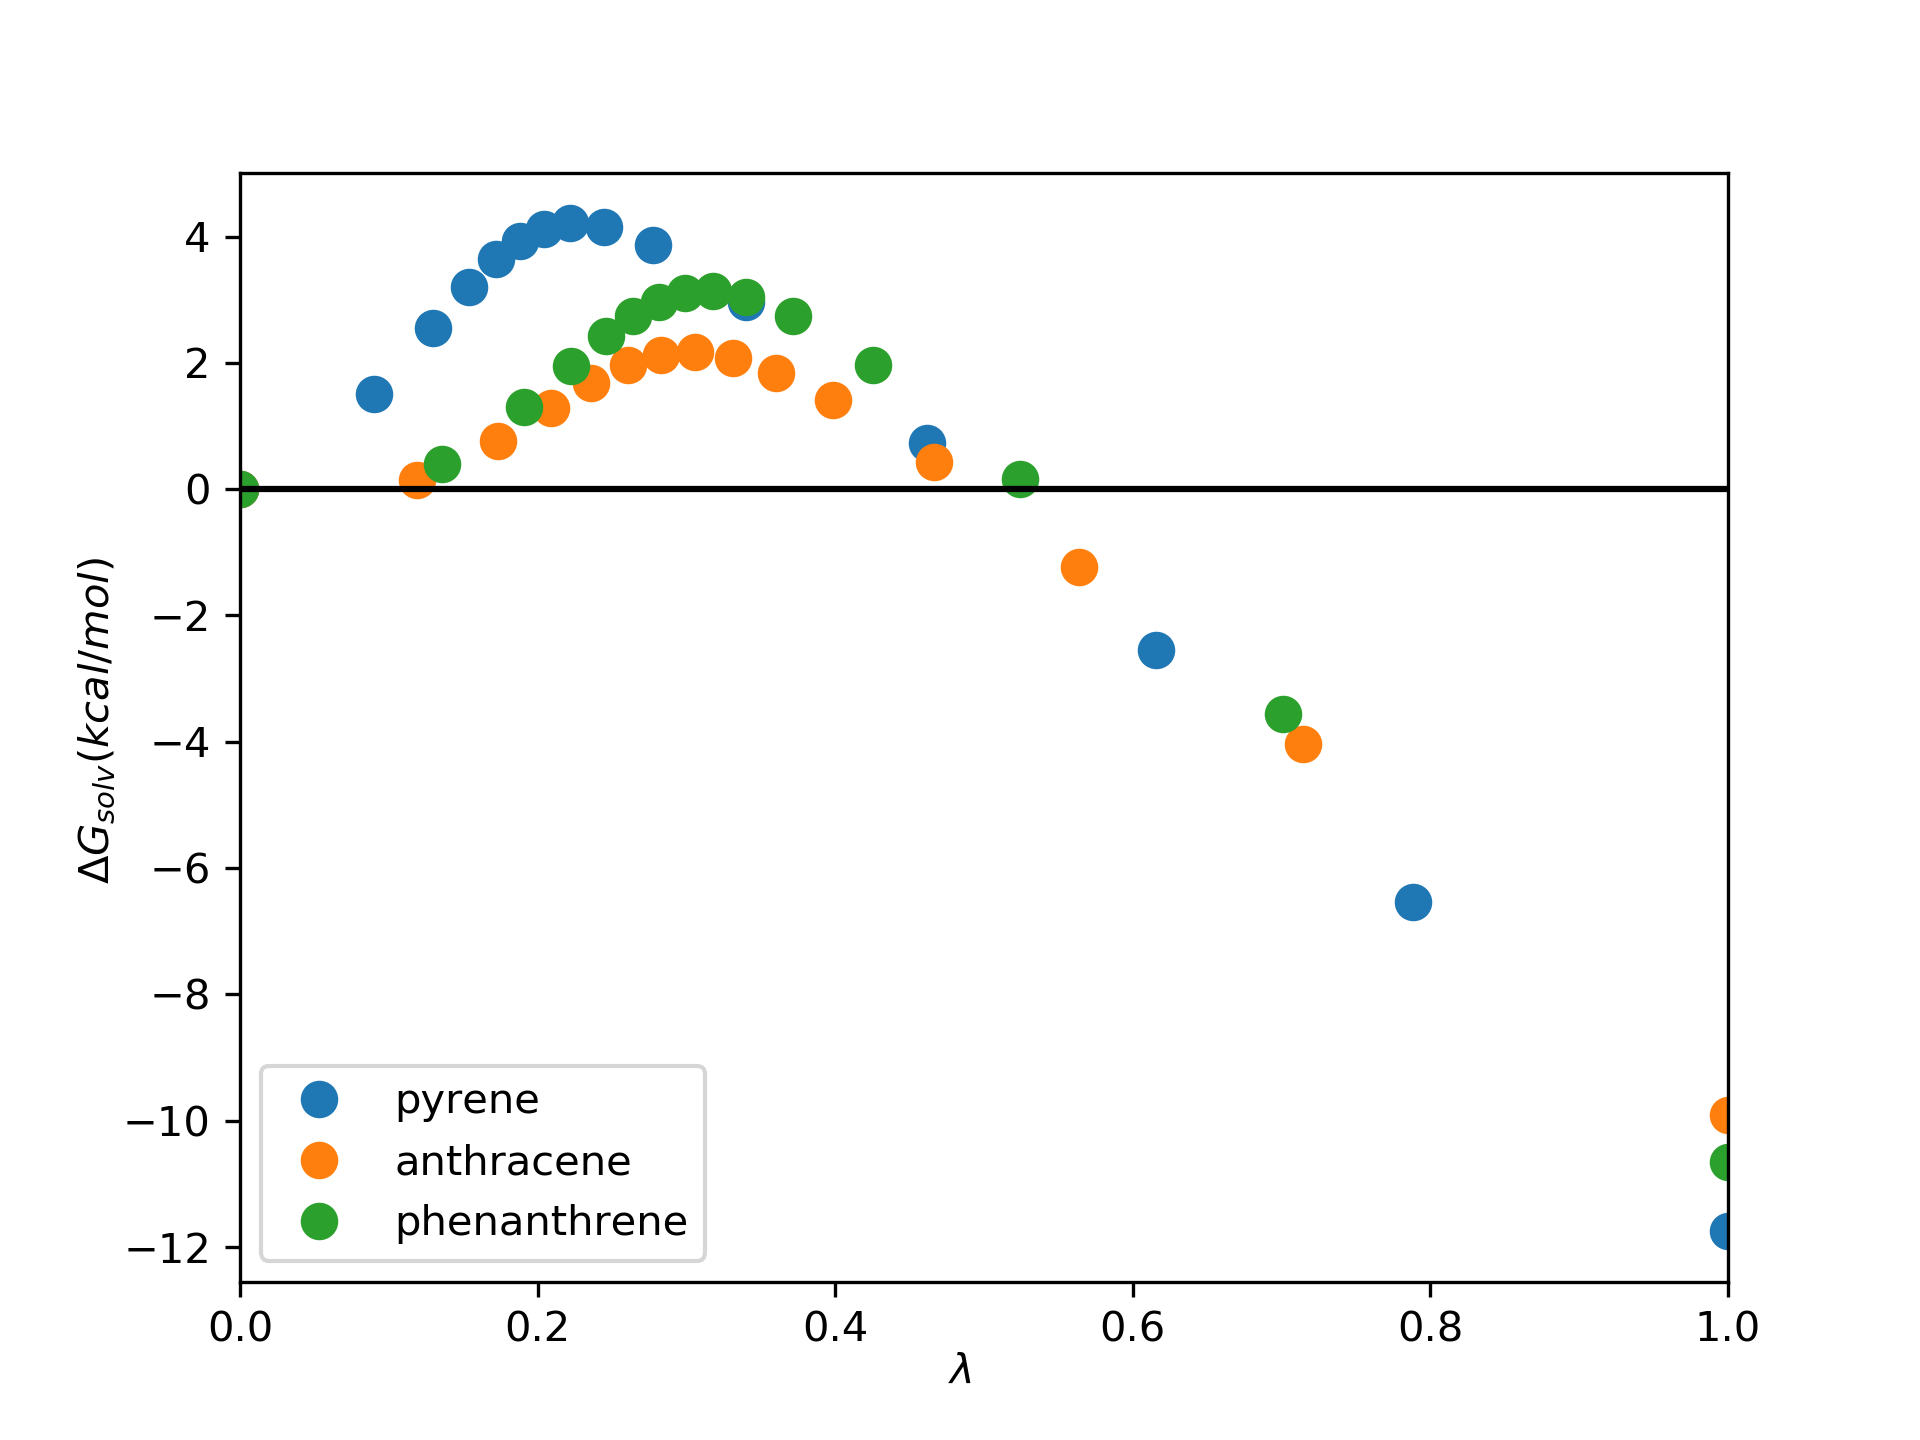
\includegraphics[width=0.9\linewidth]{Figures/tol}
    \caption{Solvation free energy profiles of different solutes in toluene. }
    \label{fig:tol}
\end{figure}

 The results also indicated the prediction capability of the force field for pairs of aromatic solute and solvent. The influence of the molecule's geometry on the free energy curves was the same as the one observed for other solvents (Figure \ref{fig:tol}). $\Delta G_{solv}$ was also calculated for phenanthrene in toluene and in toluene+$CO_{2}$. To the best of our knowledge, there were no available experimental data for these solvation free energies, but the previous results for phenanthrene in other solvents and for the pair anthracene+toluene showed that the force field is adequate to describe the solvation phenomenon of phenanthrene in an aromatic solvent. The results for these sets are exposed below: 
 
\FloatBarrier
\begin{table}[H]
\centering
  \caption{Calculated values for the solvation free energy differences (kcal/mol) of phenanthrene in toluene+$CO_{2}$.}
  \label{tbl:solv3}
  \begin{tabular}{ll}
    \hline
    \hline
      $w_{CO_{2}}$ & $\Delta G_{solv}^{Mie}$ \\
    \hline
    0.0    & -10.65 $\pm$ 0.02   \\
    0.087  & -10.73 $\pm$ 0.02   \\
    0.119  & -10.78 $\pm$ 0.02   \\
    0.169  & -10.71 $\pm$ 0.02   \\
    0.289  & -10.69 $\pm$ 0.02   \\
    \hline
    \hline
  \end{tabular}
\end{table}
\FloatBarrier

The increase of $CO_{2}$ mass fraction in toluene caused a small effect on solvation free energies. First, the $\Delta G_{solv}$ decreased with the increase of $w_{CO_{2}}$. After the 0.119 fraction, the effect was reversed and carbon dioxide became an anti-solvent. \citeonline{SOROUSH2014405} reported that asphaltene precipitation occurs when carbon dioxide mass fractions became higher than 0.10 in the system asphaltene+toluene+carbon dioxide, what is in agreement with the anti-solvent effect of carbon dioxide observed on the calculated values. It is also important to point out that the small differences observed in the free energy profiles (Figure \ref{fig:Figure_1}) may indicate the insignificance of $CO_{2}$ in the solvation of phenanthrene in toluene when using the Saft-$\gamma$ Mie force field. But, more studies need to be done to make a secure assertion about it since this is a qualitative study due to the lack of experimental data.   

\begin{figure}[H]
\centering
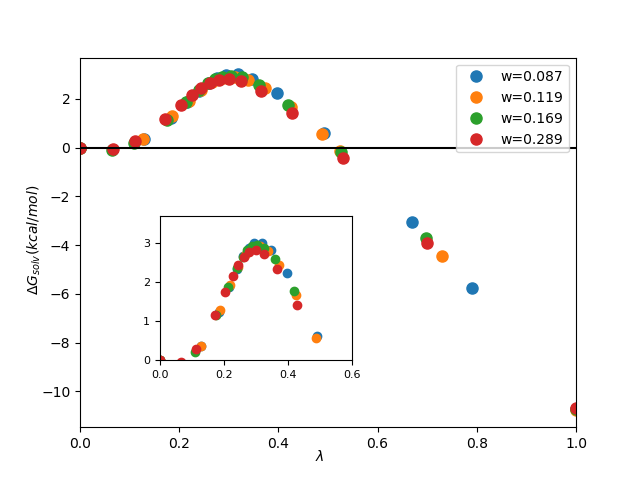
\includegraphics[width=0.9\linewidth]{Figures/Figure_1}
\caption{Solvation free energy profiles of phenanthrene in toluene+$CO_{2}$.}
\label{fig:Figure_1}
\end{figure}


\section{Hydration free energies}

We also calculated the hydration free energies of widely studied solutes (propane, benzene) and aromatic solutes (toluene, phenanthrene) with a group of fifteen intermediate states. First, the binary interaction parameter was set to zero, but the preliminary results for hydration free energies, exposed in Table \ref{tbl:solv3},  had a high deviation from the experimental data \cite{P29900000291, doi:10.1021/ct050097l}.

\FloatBarrier
\begin{table*}[h]
    \centering
    \caption{Calculated values using $k_{ij}=0$ and experimental values for the hydration free energy differences (kcal/mol) of solutes in water.}
    \label{tbl:solv3}
    \begin{tabular}{llll}
    	\hline\hline
    	Solute       & $\Delta G_{solv}^{exp}$ & $\Delta G_{solv}^{Mie}$ & Absolute Deviation \\ \hline
    	propane      & 2.00 $\pm$ 0.20         & 1.10 $\pm$ 0.01         & 0.90               \\
    	benzene      & -0.86 $\pm$ 0.20        & -4.45 $\pm$ 0.03        & 3.59               \\
    	toluene      & -0.83 $\pm$ 0.20        & -10.98 $\pm$ 0.30       & 10.15              \\
    	phenanthrene & -3.88 $\pm$ 0.60        & -10.90 $\pm$ 0.04       & 7.02               \\ \hline\hline
    \end{tabular}
\end{table*}
\FloatBarrier

After these results, the need for binary interaction parameters was clear. First, we estimated $k_{ij}$ with the SAFT VR Mie EoS and experimental vapor pressure data, but this strategy also did not provide good results. Hence, we used the approach of estimating the $k_{ij}$ with the output from solvation free energy calculations with molecular dynamics, as described in the last paragraph of section \ref{solvme}.  We initially found individual values for the interaction parameter of each pair, but, since the parameters for aromatic solutes were very similar (0.148, 0.162, 0.152), we averaged these values. By doing that,  we obtained a general parameter for the water+aromatic pairs:

\begin{table*}[h]
  \centering
  \caption{Binary interaction parameters employed.}
  \label{tbl:kij}
  \begin{tabular}{ll}
    \hline
    \hline
      Pair & $k_{ij}$ \\
    \hline
    water  + propane      & 0.067  \\
    water  + aromatic      & 0.154 \\  
    \hline
    \hline
  \end{tabular}
\end{table*}

The relatively large $k_{ij}$ value of the aromatic solutes can be pinned on the lack of an explicit association term in the model and on the water model itself since the force field did not need a $k_{ij}$ for mixtures with the other hydrogen bonding solvent (1-octanol).  This SAFT-$\gamma$ Mie model for water \cite{lobanova2016} has two different temperature-dependent sets of parameters. The parameters utilized in this work was the one estimated with experimental interfacial tension data. Hence, we tested the binary interaction parameter for water+toluene estimated with MD interfacial data by \citeonline{herdes2017}. Nevertheless, the result was not satisfactory and this parameter could not be transferable to the solvation free energy of toluene in water. 

These issues faced by SAFT-$\gamma$ Mie model are related to the problems of modeling water with a coarse-grained force field. One of the main difficulties is the choice of which water molecules are going to be represented by which specific beads since water molecules move independently and are only bound by non bonded interactions \cite{hadley2010,hadley2012}. The  SAFT-$\gamma$ Mie water considers that one water molecule corresponds to one bead. This strategy only saves small simulation time, but it can predict properties at physiological temperatures unlike other more aggressive models, which consider that one bead represents various water molecules. In light of all this, the SAFT-$\gamma$ Mie force field appears to be a good alternative when working close to room temperatures, but the necessity of additional parameters estimated with molecular simulation indicates problems on the model. Using these parameters, we then obtained the final hydration free energy differences presented in Table \ref{tbl:solv2}. 

\begin{table}[H]
  \centering
  \caption{Calculated and experimental hydration free energy differences  (kcal/mol) of solutes in water.}
  \label{tbl:solv2}
  \begin{tabular}{llllll}
  	\hline\hline
  	Solute       & $\Delta G_{solv}^{GAFF}$ & $\Delta G_{solv}^{ELBA}$ & $\Delta G_{solv}^{exp}$ & $\Delta G_{solv}^{Mie}$ & Absolute  \\
  	             &                          &                          &                         &                         & Deviation \\ \hline
  	propane      & 2.50 $\pm$0.02           & 2.76 $\pm$ 0.02          & 2.00 $\pm$ 0.20         & 2.01 $\pm$ 0.01         & 0.01      \\
  	benzene      & -0.81$\pm$0.02           & -0.69 $\pm$ 0.01         & -0.86 $\pm$ 0.20        & -1.12 $\pm$ 0.01        & 0.26      \\
  	toluene      & -0.79$\pm$0.03           & -0.76 $\pm$ 0.01         & -0.83 $\pm$ 0.20        & -0.84 $\pm$ 0.01        & 0.01      \\
  	phenanthrene & -5.26$\pm$0.03           & -                        & -3.88 $\pm$ 0.60        & -3.47 $\pm$ 0.02        & 0.41      \\ \hline\hline
  	%    RMSE    &                          &                          & 0.24                    &  \\
  	%    \hline  &
  \end{tabular}

\end{table}

Hydration free energy differences calculated using the SAFT-$\gamma$ Mie force field with $k_{ij} \neq 0$ had low absolute deviations to the experimental data, as expected since the parameters were adjusted to fit the experimental data. In the table above, we also show the results obtained by \citeonline{PMID:24928188} with the GAFF force field and by \citeonline{doi:10.1021/acs.jctc.5b00963} with the ELBA force field. The GAFF (General Amber Force Field) force field is an all-atom model that consists of bonded and non bonded parameters and is suitable for the study of a significant number of molecules. Meanwhile, the ELBA force field is a coarse-grained model that comprises six independent parameters. This force field models three carbons as one Lennard-Jones site and one water molecules as one Lennard Jones site with a point dipole. 

Comparing the three force fields, the root mean square error (RMSE) for the pairs tested with the SAFT-$\gamma$     Mie model was  0.24, the RMSE for hydration free energy differences with the GAFF force field was 0.73, and the RMSE for the ELBA coarse-grained force field was 0.44. The difference in absolute deviations between the GAFF and SAFT-$\gamma$     Mie force fields is significantly high for phenanthrene, hence the coarse-grained force field with a binary parameter is preferred if the application requires a higher level of accuracy. The results also indicated that the SAFT-$\gamma$ Mie Model with the binary interaction parameter performed better than the ELBA force field in modeling the solvation phenomenon of the pairs studied in this work and worst with the binary parameter equal to zero. This fact occurred despite the fact that both models have the same level of coarse-graining (one bead represents one water molecule). Hence, the choice between the two coarse-grained models is dependent on the availability and transferability of binary interaction parameters for the Mie Model. We also present, for the SAFT-$\gamma$ Mie force field, the hydration free energy profiles in Figure \ref{fig:water}. The geometry dependence on the free energy profiles is apparent as it was for the solvation free energy study in other solvents. We also observe that the hydration free energy for the first non zero $\lambda$ is negative for benzene and toluene when a positive value is expected since energy is required to 'open space' in the solvent for the solute's insertion. This anomaly can be caused by numerical errors during the estimation or by another inconsistency in the force field. 

\begin{figure}[H]
\centering
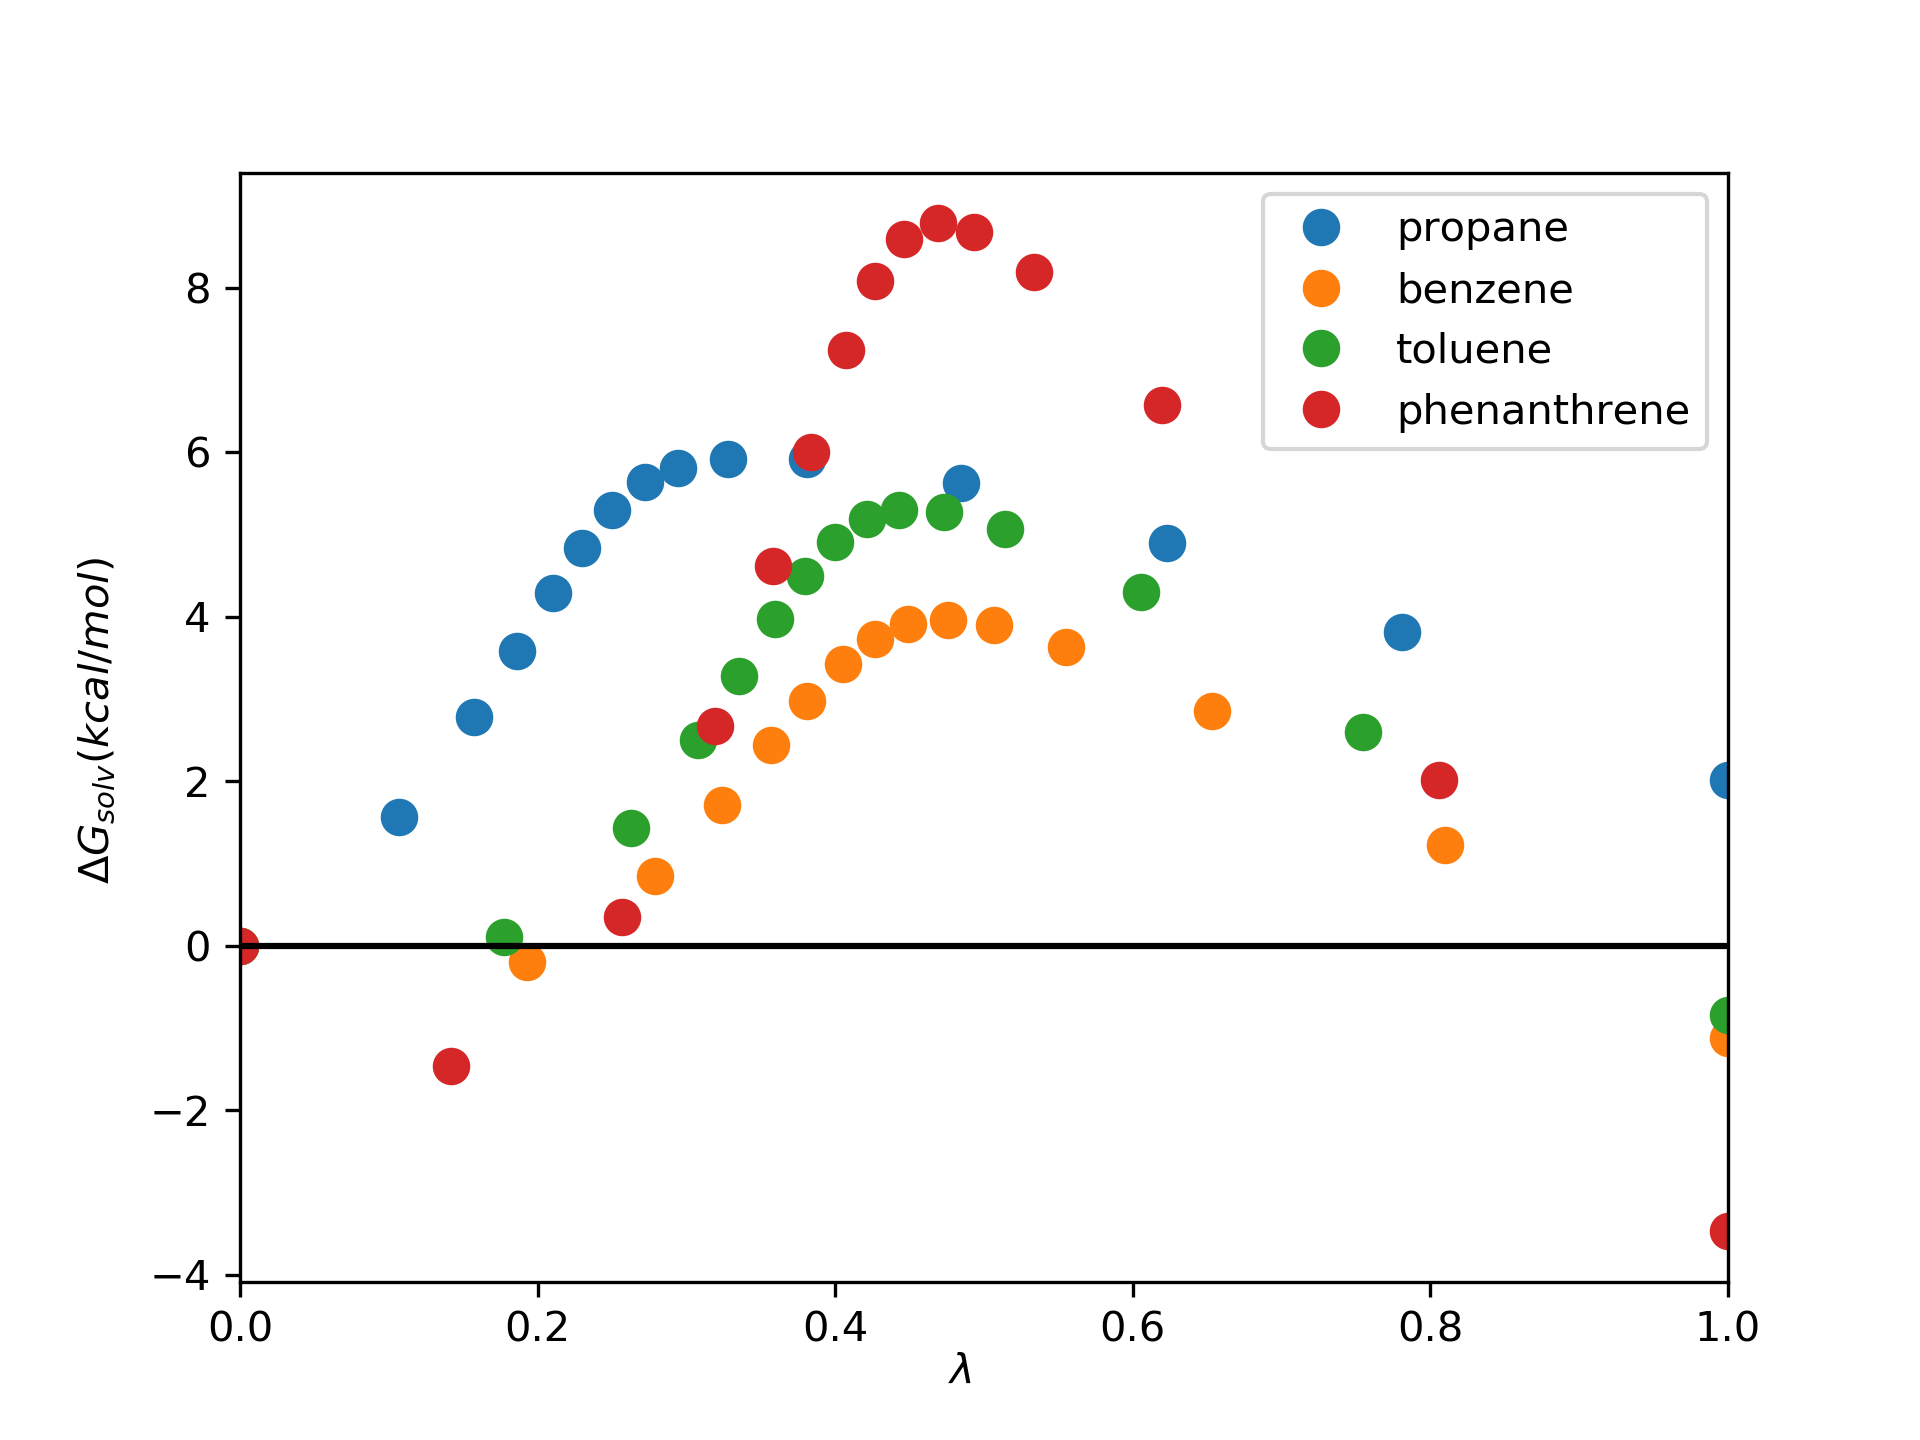
\includegraphics[width=0.9\textwidth]{Figures/water}
\caption{Hydration free energy profiles for different solutes.}
\label{fig:water}
\end{figure}

\section{Partition Coefficients}

Using the solvation free energies estimated in the sections above, we also calculated partition coefficients, Eq. \eqref{eqn:partcoe}, for toluene/hexane, water/hexane, and water/1-octanol. The later is the one with most experimental data in the literature because 1-octanol is used to quantify hydrophobicity and it can serve as a model for biological lipids and different soils \cite{RUELLE2000457}. Our interest in calculating the other two coefficients is due to the use of hexane as a model for an apolar, hydrophobic phase and because of the characterization of asphaltenes by hexane and toluene. Calculated values and experimental data are in Table \ref{tbl:part}. The experimental data of partition coefficients  were only available for water/1-octanol  \cite{POOLE2000117,sangster} and water/hexane \cite{doi:10.1021/je970112e}. Hence, for the partition coefficient of toluene/ hexane, we used the solvation free energy experimental data exposed in Table \ref{tbl:solv1} as input in Eq. \eqref{eqn:partcoe} to generate estimated experimental data.


\begin{table}[H]
    \centering
    \caption{Partition Coefficient Calculated from MD simulations and from experimental data.}
    \label{tbl:part}
    \begin{tabular}{llll}
    	\hline\hline
    	             & {Molecular Dynamics} & {Experimental} & Absolute Deviation \\ \hline
    	              \multicolumn{4}{c}{log $P^{water/1-octanol}$}               \\ \hline
    	propane      & 2.47                 & 2.40           & 0.07               \\
    	phenanthrene & 3.57                 & 4.46           & 0.89               \\ \hline
    	               \multicolumn{4}{c}{log $P^{water/hexane}$}                 \\ \hline
    	benzene      & 1.93                 & 2.06           & 0.13               \\
    	phenanthrene & 4.17                 & 4.49           & 0.32               \\ \hline
    	               \multicolumn{4}{c}{log $P^{tolune/hexane}$}                \\ \hline
    	pyrene       & -0.67                & -0.97          & 0.30               \\
    	phenanthrene & -0.47                & -              & -                  \\ \hline\hline
    \end{tabular}
    
\end{table}

Overall absolute deviations were small for pairs with smaller solvation free energy deviations such as propane and benzene. The water/1-octanol partition coefficient of phenanthrene had higher deviation due to the higher deviation of the free energy of solvation of this compound in 1-octanol. The toluene/hexane partition coefficient of pyrene has its high deviation related to the prediction of the solvation free energy in toluene. Comparing with other force fields, \citeonline{garrido} reported average absolute deviations for the water/1-octanol partition coefficient of 0.4 for Gromos, 0.3 for TraPPE and 0.9 for OPLS-AA/TraPPE force fields. However, they attribute the low deviations of TraPPE to the cancellation of errors between the two solvation free energies. Additionally, \citeonline{doi:10.1021/acs.jctc.5b00963} found average absolute deviations of 0.86 for the water/hexane partition coefficient and of 0.75 for the water/1-octanol partition coefficient with the ELBA coarse-grained force field. Although these papers did not predict the partition coefficient of phenanthrene and pyrene in the pair of solvents, we can say that the predictions for our small sets of solute-solvent stayed in the same overall range of absolute deviations observed for the other predictions in this work. However, a larger set would be necessary to do a complete evaluation of this force field using partition coefficients. 